\section{Chapter 9}
%TODO:C-9.3
%TODO:C-9.14

\begin{itemize}
    \item[R-9.1]  Which of the hash table collision-handling schemes could tolerate a load
          factor above 1 and which could not?

          \answer Seperate chaining can tolerate a load factor above 1 but none of the
          open addressing schemes can.

    \item[R-9.6]  Describe how to use a skip-list map to implement the dictionary ADT,
          allowing the user to insert different entries with equal keys.

          \answer Have the entries be stored in a bucket and when a entry with a key already
          in the skip list is inserted, have it be added to the bucket. Of course you would have
          to update all levels of the skiplist. Then for findAll have a range class nested in the
          dicionary class and return a range that contains all entries that have that key.

    \item[R-9.7]  Draw the 11-entry hash table that results from using the hash function,
          h(i) = (3i + 5) mod 11, to hash the keys 12, 44, 13, 88, 23, 94, 11, 39, 20,
          16, and 5, assuming collisions are handled by chaining.

          \answer
          \begin{center}
              \begin{tabular}{|l|*{11}{c|}}
                  \hline
                  Index & 0  & 1      & 2 & 3 & 4 & 5          & 6 & 7 & 8      & 9     & 10 \\
                  \hline
                  Key   & 13 & 94, 39 &   &   &   & 44, 88, 11 &   &   & 12, 23 & 16, 5 & 20 \\
                  \hline
              \end{tabular}
          \end{center}

    \item[R-9.8] What is the result of the previous exercise, assuming collisions are handled
     by linear probing?

          \answer
          \begin{center}
              \begin{tabular}{|l|*{11}{c|}}
                  \hline
                  Index & 0  & 1  & 2  & 3  & 4 & 5  & 6  & 7  & 8  & 9  & 10 \\
                  \hline
                  Key   & 13 & 94 & 39 & 16 & 5 & 44 & 88 & 11 & 12 & 23 & 20 \\
                  \hline
              \end{tabular}
          \end{center}

    \item[R-9.10]  What is the result of Exercise R-9.7 when collisions are handled by double
          hashing using the secondary hash function $h` (k) = 7 - (k \ mod\  7)?$

          \answer
          \begin{center}
              \begin{tabular}{|l|*{11}{c|}}
                  \hline
                  Index & 0  & 1  & 2  & 3  & 4  & 5  & 6 & 7  & 8  & 9  & 10 \\
                  \hline
                  Key   & 13 & 94 & 23 & 11 & 39 & 44 & 5 & 88 & 12 & 16 & 20 \\
                  \hline
              \end{tabular}
          \end{center}

    \item[R-9.14] Explain why a hash table is not suited to implement the ordered dictionary ADT.

          \answer A hash table isn't suited to implement the ordered dictionary ADT because by putting keys
          through a hash function doesn't preserve order because it compresses the keys.

    \item [R-9.15] What is the worst-case running time for inserting n items into an initially
          empty hash table, where collisions are resolved by chaining? What is the
          best case?

          \answer The worst case is $\mathcal{O}(n^2)$ where each key is mapped to to the same bucket.
          It will take one probe for the first, two for the second and so on until the $n^{\text{th}}$
          probe. The best case running time is $\mathcal{O}(n)$ where every key maps to a different index.

    \item[R-9.16] Draw an example skip list that results from performing the following
          series of operations on the skip list shown in Figure 9.12: erase(38),
          insert(48, x), insert(24, y), erase(55). Record your coin flips, as well.

          \answer \\
          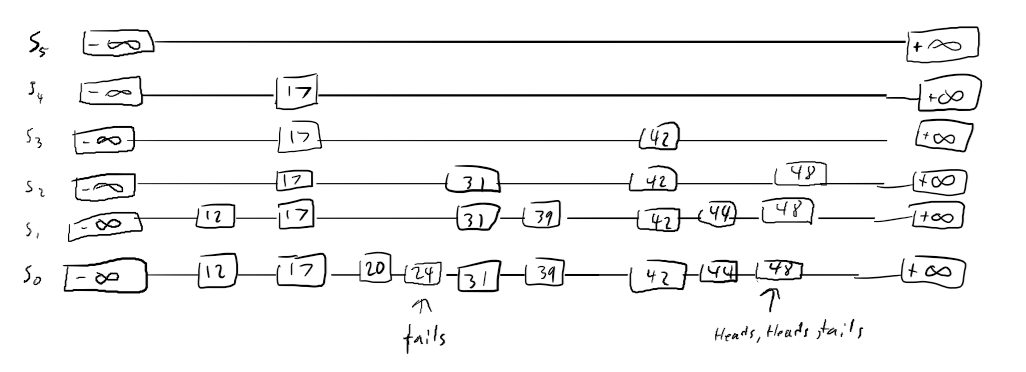
\includegraphics[scale=.6]{img/R_9_16_skiplist.png}
          \newpage

    \item[C-9.3] Suppose we are given two ordered dictionaries S and T , each with n items,
          and that S and T are implemented by means of array-based ordered sequences.
          Describe an $O(\log^2n)$-time algorithm for finding the kth smallest key in the union
          of the keys from S and T (assuming no duplicates).

          \answer First we can ignore all indices greater than k in both arrays.

    \item[C-9.5] Design a variation of binary search for performing findAll(k) in an ordered
          dictionary implemented with an ordered array, and show that it runs in
          time $O(\log n + s)$, where n is the number of elements in the dictionary and
          s is the size of the iterator returned.

          \answer Do normal binary search until you find the index that holds the key you
          are searching for. To then get the range of indices to return make 2 loops, one
          that decreases the index until it reaches a new key at index i, and one that increases the
          index until it finds a new key at index j. The range would then be indices i+1 through j-1.
          This runs in $O(\log n + x)$ because the initial search is is $O(\log n)$ and finding the range
          is $O(s)$.

    \item[C-9.14] Describe an efficient data structure for implementing the bag ADT, which
          supports a function add(e), for adding an element e to the bag, and a
          function remove, which removes an arbitrary element in the bag. Show
          that both of these functions can be done in O(1) time.

          \answer We can use an array with 2 member variables, index and last. Index will keep track of 
          of where we are inserting into the array. It will start at zero and increment after insertion and
          last will be the index of the last inputted item. This means that insertion will be $O(1)$. Now for removal
          we will accept some index to remove. We will copy last over to that index effectively erasing it and then 
          decrement both last and index by one. This is also done in constant time.













\end{itemize}